%%%%%%%%%%%%%%%%%%%%%%%%%%%%%%%%%%%%%%%%%%%%%%%%%%%%%%%%%%%%%%%%%%%%%%%%%%%%%
%
%  System        : 
%  Module        : 
%  Object Name   : $RCSfile$
%  Revision      : $Revision$
%  Date          : $Date$
%  Author        : $Author$
%  Created By    : Robert Heller
%  Created       : Wed May 31 20:09:46 2017
%  Last Modified : <171103.2144>
%
%  Description 
%
%  Notes
%
%  History
% 
%%%%%%%%%%%%%%%%%%%%%%%%%%%%%%%%%%%%%%%%%%%%%%%%%%%%%%%%%%%%%%%%%%%%%%%%%%%%%
%
%    Copyright (C) 2017  Robert Heller D/B/A Deepwoods Software
%			51 Locke Hill Road
%			Wendell, MA 01379-9728
%
%    This program is free software; you can redistribute it and/or modify
%    it under the terms of the GNU General Public License as published by
%    the Free Software Foundation; either version 2 of the License, or
%    (at your option) any later version.
%
%    This program is distributed in the hope that it will be useful,
%    but WITHOUT ANY WARRANTY; without even the implied warranty of
%    MERCHANTABILITY or FITNESS FOR A PARTICULAR PURPOSE.  See the
%    GNU General Public License for more details.
%
%    You should have received a copy of the GNU General Public License
%    along with this program; if not, write to the Free Software
%    Foundation, Inc., 675 Mass Ave, Cambridge, MA 02139, USA.
%
% 
%
%%%%%%%%%%%%%%%%%%%%%%%%%%%%%%%%%%%%%%%%%%%%%%%%%%%%%%%%%%%%%%%%%%%%%%%%%%%%%

\chapter{MCP23017Hat: 16 bit GPIO expander HAT}

This is a circuit board to for an add-on board for a Raspberry Pi B+ that will 
add 16 3V GPIO pins, using a MCP23017 I2C I/O expander. There is a jumper 
header to set one of eight addresses for the MCP23017 chip.  This allows using 
more than one of this board or any other board featuring a MCP23008 or 
MCP23016 or MCP23017 chip (up to eight total). 

The circuit board uses a 40pin header socket to connect to the 40pin header on 
the  Raspberry Pi B+ and can use a  stack-through  header to allow  additional 
boards to be stacked on top of it.                                             
 
\section{Circuit Description}          

\begin{figure}[hbpt]\begin{centering}%
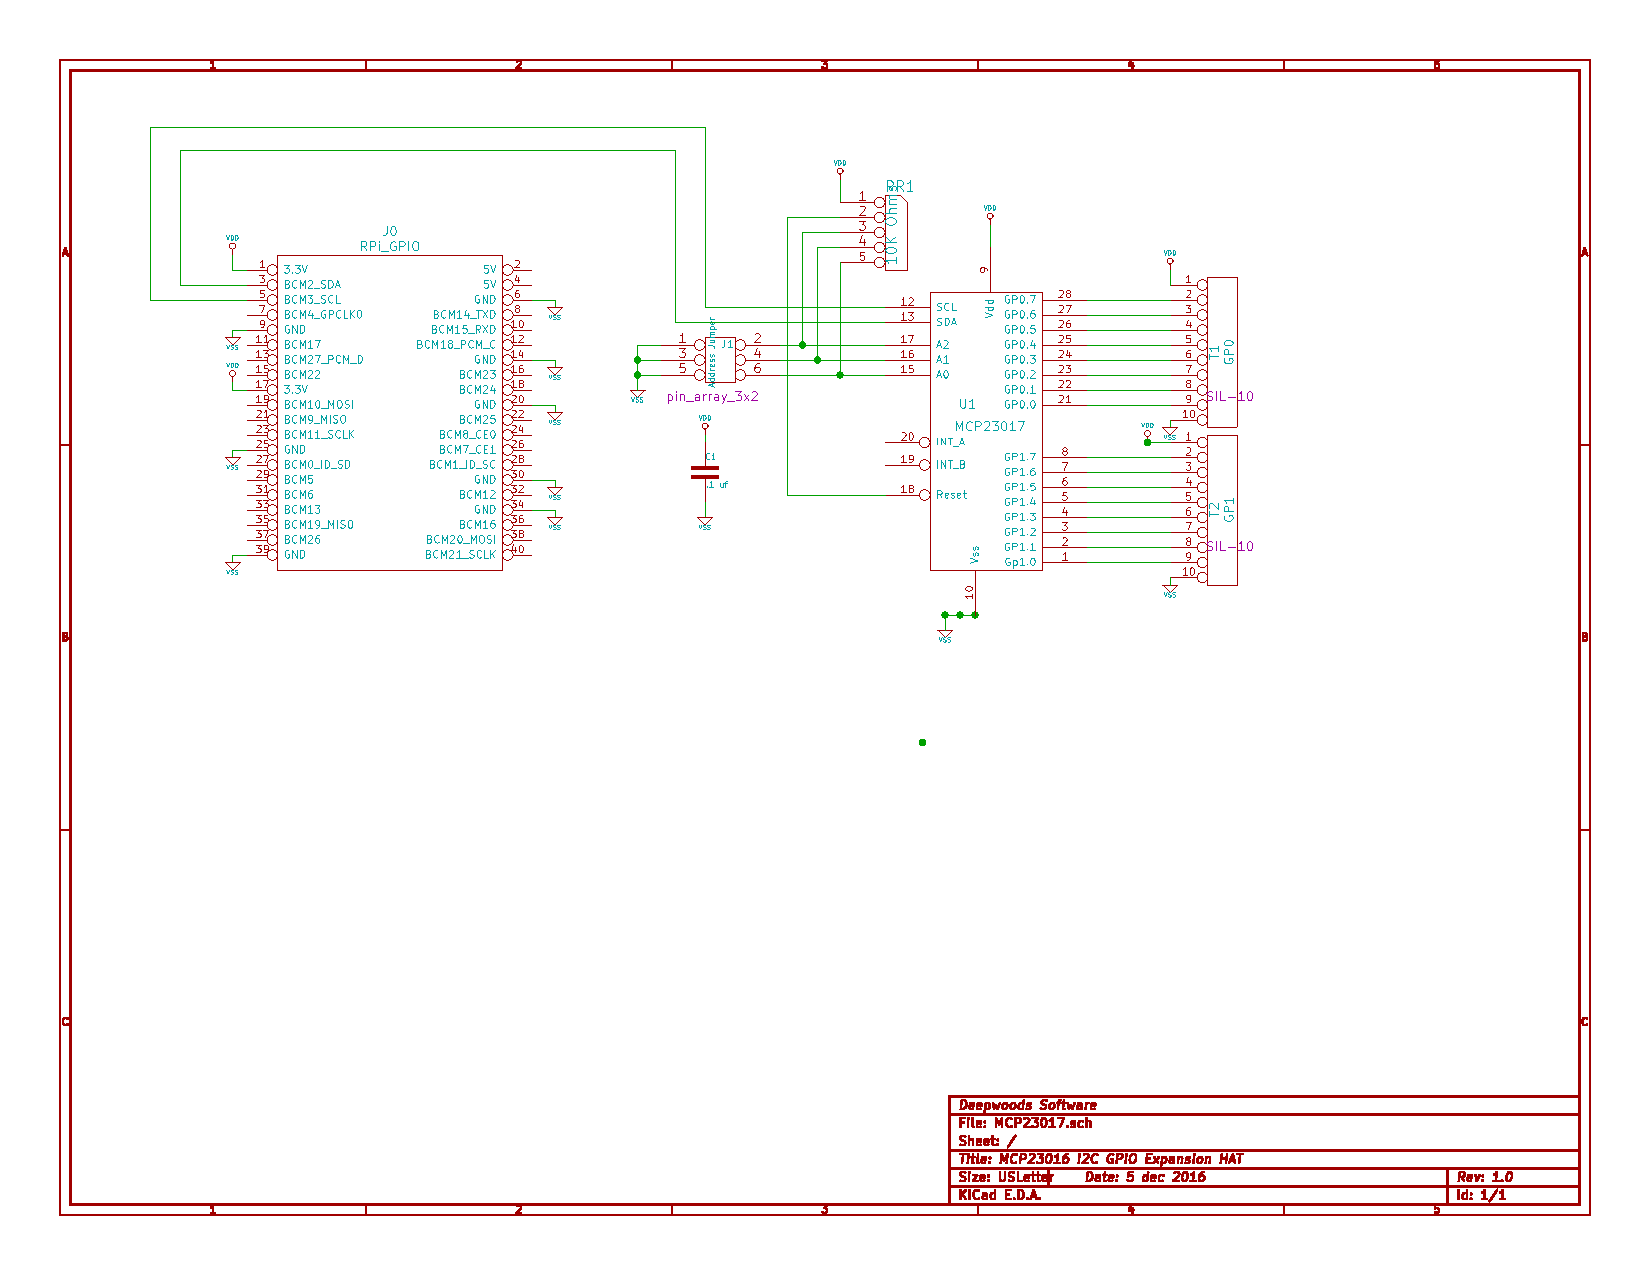
\includegraphics[width=5in]{MCP23017.pdf}
\caption{Circuit Diagram of the MCP23017}
\end{centering}\end{figure}
This circuit uses a MCP23017 to expand the Raspberry Pis I/O to 16 additional 
I/O pins. The 16 3V logic pins are simply brought out to screw terminals, 
along with the 3V and ground connections (useful for logic reference).

\section{Parts List}

\begin{table}[htdp]
\begin{centering}\begin{tabular}{|l|l|p{1in}|l|p{.5in}|}
\hline
Value&Qty&Refs&Mouser Part Number&Adafruit Part Number\\
\hline
.1 uf&1&C1&21RZ310-RC&\\
\hline
RPi GPIO&1&J0&855-M20-6102045&2223\\
\hline
Address Jumper&1&J1&517-929836-02-03&\\
\hline
10K Ohms&1&RR1&652-4605X-1LF-10K&\\
\hline
GP0;GP1&2&T1 T2&651-1725737 or 2x 651-1725685&\\
\hline
MCP23017&1&U1&579-MCP23017-E/SP&\\
\hline
\end{tabular}
\caption{Parts list for MCP23017 boards.}
\end{centering}\end{table}\footnote{Mouser Project link: 
\url{http://www.mouser.com/ProjectManager/ProjectDetail.aspx?AccessID=25df06786a}.}

The only parts that might be substituted are J0 (the RPi GPIO Header), and T1
and T2 (the I/O terminals). The parts listed are for the stacking headers for 
the RPi GPIO Header, and screw terminals for the I/O terminals.  Feel free to 
select a non-stacking header for the RPi GPIO Header and to select either pin 
arrays or spring terminals for the T1 and T2.                   

\section{Circuit Board Layout}

\begin{figure}[hbpt]\begin{centering}%
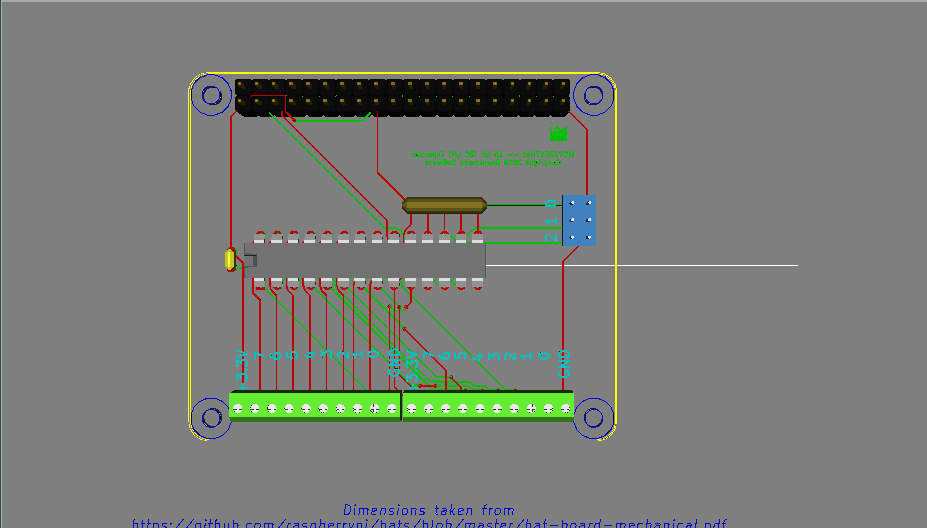
\includegraphics[width=5in]{MCP230173DTop.png}
\caption{3D rendering of the MCP23017 board}
\end{centering}\end{figure}
\begin{figure}[hbpt]\begin{centering}%
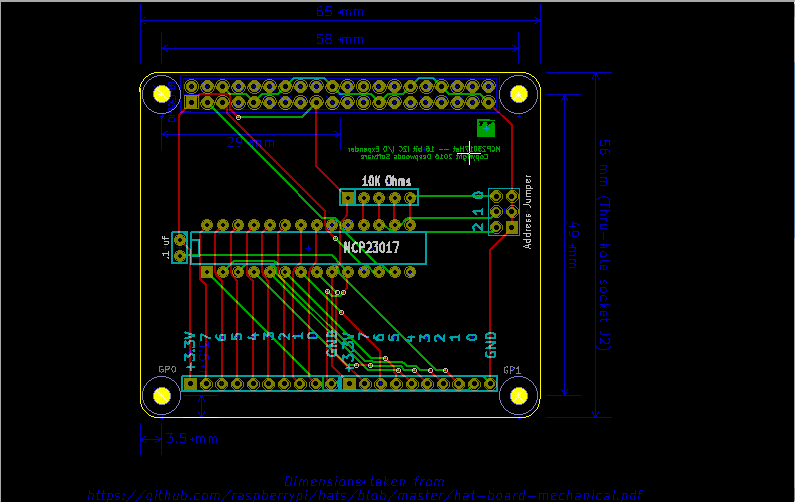
\includegraphics[width=5in]{MCP23017.png}
\caption{Fabrication image of the MCP23017 board}
\end{centering}\end{figure}
Board assembly is straight forward. You need to be careful orienting the IC.
Also the SIP resistor array needs to be carefully oriented -- the dot marks
pin 1, which is indicated on the board with a square pad. 

\section{Downloadables and Software Support}

Full design information is available on GitHub here:
\url{https://github.com/RobertPHeller/RPi-RRCircuits/tree/master/MCP23017Hat}.

This board is supported by the Model Railroad System
\texttt{OpenLCB\_PiMCP23017} and \texttt{OpenLCB\_PiMCP23017\_signal} daemons.
A basic XML file for it is included in its GitHub folder. 


